%!TEX root = ../doc.tex
\chapter{Testing and Results}
\label{sec:Results}
The following chapter describes the calibration, testing and the results of the system components. 
\section{ToF Camera}
The time-of-flight camera is the main part of this thesis, allowing a three-dimensional scene reconstruction. This section describes the measurements and the results of the motion estimation using this camera at every involved step.
\subsection{Setup}
As described in Section \ref{sec:camHead}, the ToF camera sends its data by ethernet, using a lightweight TCP protocol. The software controlling the setup of the ToF camera runs on the Raspberry Pi and is the proprietary part of the ToF software stack. The software allows a basic configuration in two main modes: automatic and manual control. The software supports HDR functionality in both automatic and manual control, which significantly enhances the dynamic range on the infrared black-and-white image.\\ 
The ToF camera uses an infrared flash, which is not brightness-controlled. Setting the camera to a fixed exposure time would lead to overexposure on close objects. The automatic mode lets the user select a maximum amplitude of the image, to which the exposure time is set. As the CudaSift library, which extracts the SIFT features from the ToF camera, only supports the 8-bit resolution, the maximum amplitude was set to 255. Higher values lead to a longer exposure time and let the frame rate drop. Not needing any amplitude scaling while keeping a high frame rate is favorable.\\
The coordinate system is not corrected for $x$, $y$ and $z$ yet, as the ToF camera itself does not know its rotation in the field of gravity. Therefore, the axis for the ToF camera calculations are kept in the $a$, $b$ and $c$ system. Details are explained in Section \ref{sec:ABC_XYZ_coords}.
\subsection{Distance measurement}
\label{sec:results_distance_meas}
Every pixel of a ToF camera sensor combined with the wide-area infrared flash acts like a laser rangefinder. A single pixel of the sensor targeting a brown cardboard surface positioned at various distances allows measuring this distance with a folding meter and a comparison with the sensor pixel value. Fitting a line to the measured data points gives the linear relation from the distance
\begin{equation*}
    d [m] = 0.000227 * val +0.247532
\end{equation*}
to the camera value $val$.
\begin{figure}[H]
  \centering
  \includegraphics[width=1.0\textwidth]{images/camera_distance_measurement.eps}
  \caption{Sensor values measured against a folding meter. The red curve shows a linear fit of the data points.}
  \label{im:distance_measurement}
\end{figure}
The camera noise does affect not only the black-and-white image but also the distance measurement. At the chosen camera settings, the camera noise causes the distance measurement to have an standard deviation in the $a$-axis of 7mm.\\
The formulae for the 3D scene reconstruction propagate the uncertainty to the $b$- and $c$-axes to about 4mm and 3mm respectively.
\subsection{3D Scene Reconstruction}
After calibrating the lens and correcting the radial nature of the distance measurement, as described in Section \ref{sec:ToFCalibration}, the generated point cloud directly reconstructed the three-dimensional scene recorded by the ToF camera.\\
Straight lines in the real world appear straight in the point cloud, which was veryfied by analyzing a straight line in the chosen scene using SIFT features, as shown in Figure \ref{fig:linearity3d}.
\begin{figure}[H]
    \centering
    \begin{minipage}[b]{0.47\textwidth}
      \includegraphics[scale=0.11]{images/cloud_3d_linearity_image.png}
      \subcaption{Image}
      \label{fig:linearity3d_image} 
    \end{minipage} % Hier darf keine Leerzeile zwischen den beiden Minipages liegen!
    \begin{minipage}[b]{0.47\textwidth}
      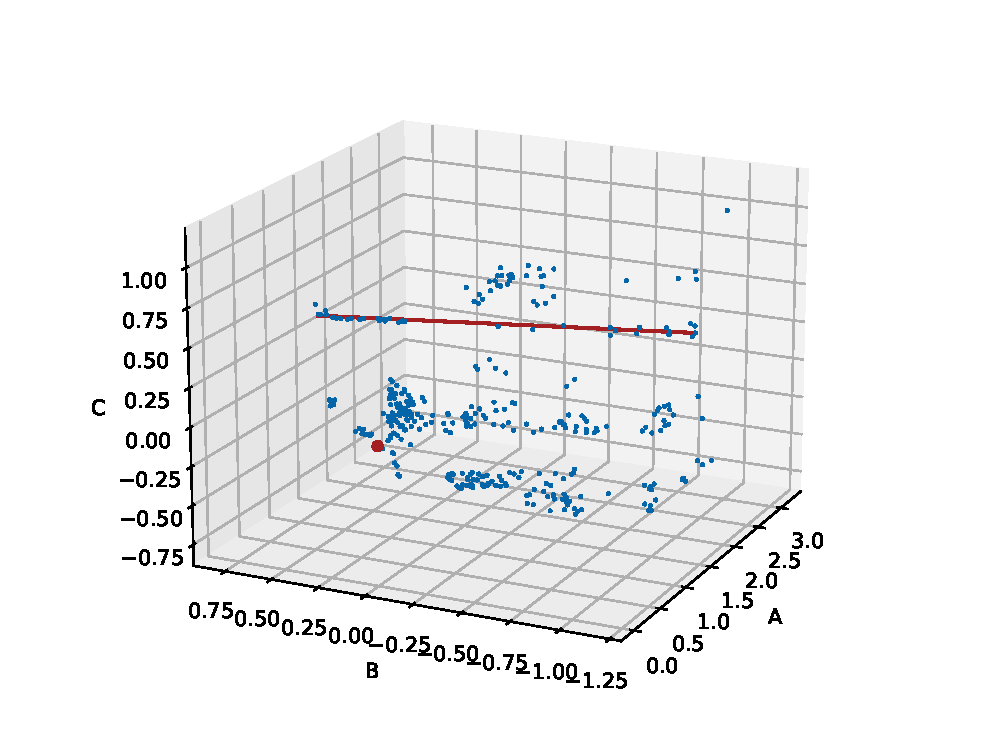
\includegraphics[scale=0.72, trim={3.3cm 3cm 3cm 3.5cm},clip]{images/linearity_3d.eps} 
      \subcaption{Cloud}
      \label{fig:linearity3d_cloud} 
    \end{minipage}
    \caption{The scene reconstruction from the left image to the full point cloud. The red line is equivalent in both figures. Each green dot in the left image is a SIFT feature. The red dot in the point cloud is the position of the camera.}
    \label{fig:linearity3d}
  \end{figure}
\newpage
\subsection{RANSAC feature matching}
\label{sec:RANSAC_Results}
The RANSAC algorithm improves the quality of matched features over the flawed brute-force matcher. The data of the ToF camera is prone to noise, the RANSAC algorithm needs to cope with positional uncertainties. As discussed in Section \ref{sec:results_distance_meas}, the standard deviation in the $a$-axis is roughly 7mm, which also affects the mapping to the$b$- and $c$-axis from the 3d reconstruction.\\
A threshold based on the sum of square differences gives the RANSAC algorithm the flexibility to create suitable matches.
The SSD creates a sphere around the estimated position. The equation of a sphere of radius $r$ follows the equation $r^{2}=x^{2}+y^{2}+z^{2}$. Setting the radius $r$ equal to the standard deviation of 7 mm on the $a$-axis results in a threshold of around 0.00005. Statistically, around 68\% of the matches should reside inside this sphere of 14 mm diameter, however the number of matches is very small as seen in Figure \ref{im:noise_against_thresh} The error on the other axis is smaller as discussed in Section \ref{sec:results_distance_meas}, this does not explain the poor matching performance at this threshold, as seen in Figure . Likely, some other source of noise diminishes the matching performance. The image noise on the black-and-white image causes the extracted SIFT features jitter. Even a jitter in the range of 1 pixel easily leads - depending on its distance - to an error of more than a centimeter. On the other hand, to detect a lateral speed of 0.1 m/s at a frame rate of approximately 10 frames per second, a shift of 1 cm needs to be detected.
\begin{figure}[H]
    \centering
    \includegraphics[width=1.0\textwidth]{images/noise_against_threshold.eps}
    \caption{Plotting the feature matching performance against different thresholds shows the quality of the RANSAC feature matcher. In blue, the raw number of unmatched features in each test, in gray the brute force matches and in red the RANSAC matches.}
    \label{im:noise_against_thresh}
\end{figure}
Higher tresholds in Figure \ref{im:noise_against_thresh} show the expected performance of the brute-force matcher in grey. The RANSAC feature detector vastly improves the matching performance, seemingly up to over 97\% at the threshold of 0.005. At a threshold of 0.005, the sphere around the expected position has more than 14cm in diameter, leading to the undesired situation of the RANSAC matcher finding feature points. The RANSAC matcher might find the same match for different unsuitable feature points. The matches are not exclusive, combined with a large threshold, it is likely that most features find a match.\\
The balance between the uncertainty and the requirements for detecting slow speeds lead to a chosen threshold of 0.0005. This threshold leads to a sphere of about 4.4 cm in diameter, which filters outliers.\\ 
Figure \ref{im:3d_features_rotation} on the next page demonstrates the matching with the chosen threshold at the example of a rotation of the camera head. Two consecutive frames generated a point cloud each. The estimated rotation and translation move each data point of one cloud to a hypothetical position. The closest data point of the other cloud around this hypothetical position is accepted if it lies within a sphere of 4.4cm diameter. 
After another calculation, these matched data points lead to the optimal rigid motion, discussed in the following sections.\\

\begin{table}[ht] \centering
	\begin{tabular}{|p{5cm}|p{3cm}|p{3cm}|p{3cm}|} \hline
		\rowcolor{gray} Measurement & Rotation & Translation X & Translation Y \\
		\hline
		Total Features (avg) & 435.9 & 400.0 & 488.4\\
		\hline
		Brute-Force Matches (avg) & 117.9 & 104.2 & 112.6  \\
		\hline
		RANSAC Matches (avg) & 280.2 & 262.5 & 284.3  \\
		\hline
	\end{tabular}
	\caption{Per-Frame average performance of the feature matching approaches}
	\label{tab:ransac_performance}
 \end{table}
 The claimed performance for the brute-force matcher is below 50\% when applied to two identical images, according to the developers of the CudaSift library.\cite{cudaSiftRepo} On noisy frames, even with motion between frames, the quality is expected to be lower.\\
 Table \ref{tab:ransac_performance} shows the performance of the RANSAC implementation in comparison to the brute-force matcher. On average an improvement of over 100\% in the number of accepted matches is achieved by running the three-dimensional RANSAC algorithm.

\begin{figure}[H]
  \centering
  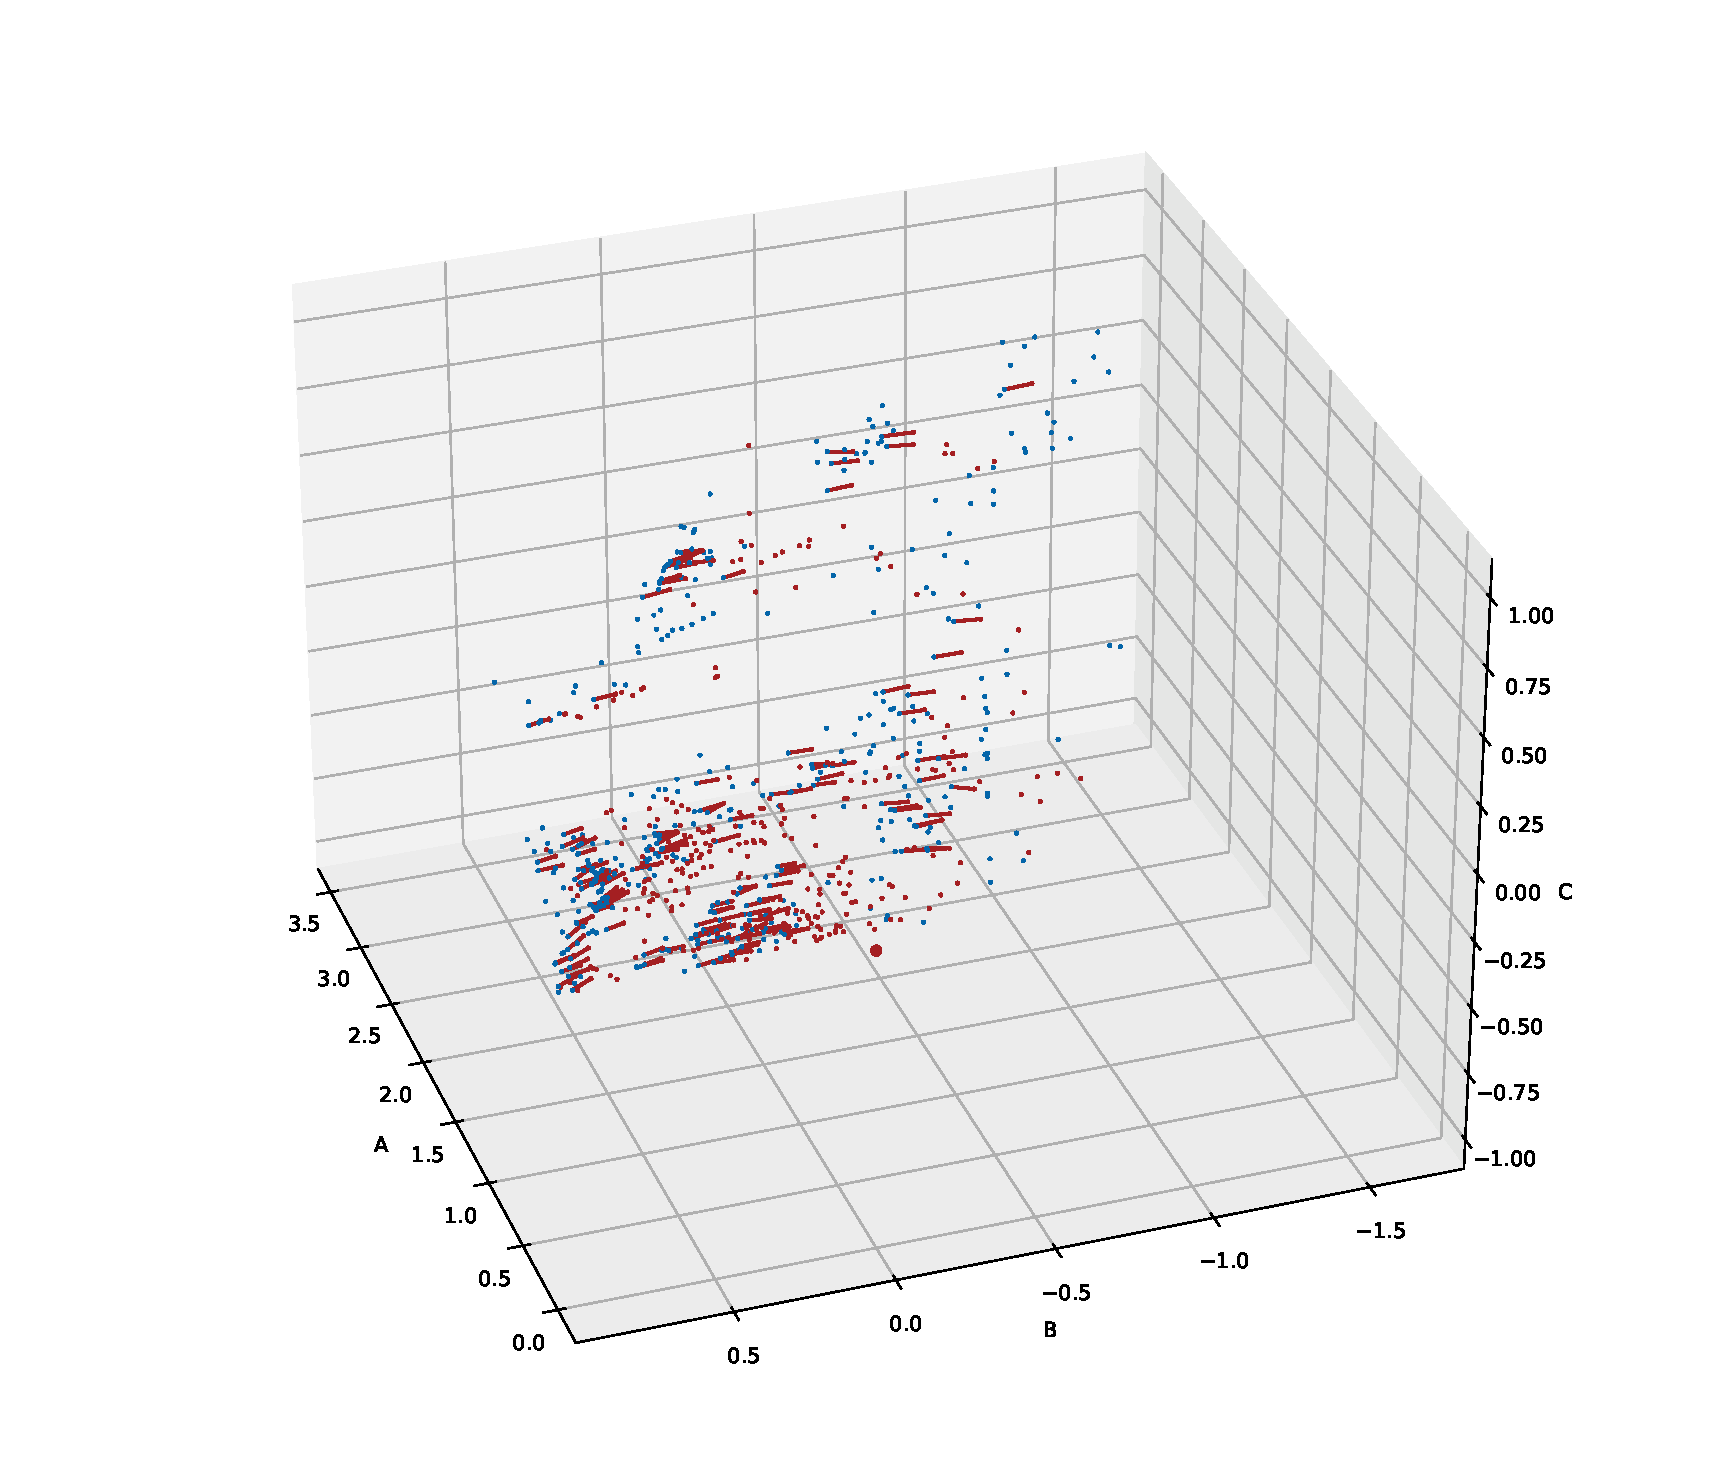
\includegraphics[width=0.97\textwidth,trim={7cm 7cm 8cm 5cm},clip]{images/3d_features_rotation.eps}
  \caption{Two raw point clouds with the found matches connecting them. The camera is rotated in between the frames, which leads to the displacement of the point cloud. The connecting lines are roughly 10cm long, depending on the position. The large red dot in the foreground is the position of the camera.}
  \label{im:3d_features_rotation}
\end{figure}
\subsection{Rotation from ToF camera}
\label{sec:results_tof_rotation}
Both the gyroscope and the ToF rotation generate rotation speeds and are both converted into rotation quaternions. Transforming the rotation speed to a quaternion allows direct comparison of the two sensory systems. Analyzing the imaginary parts is sufficient, as explained in Section \ref{sec:RotationQuaternion}.
In this experiment, the camera head was rotated in each direction and directly compared to the gyroscope data. The camera was mounted on a standard camera tripod and rotated by hand, as the author has no access to a device allowing automated rotations. Figure \ref{im:tof_rotation_measurement} shows the results. 
\begin{figure}[H]
  \centering
  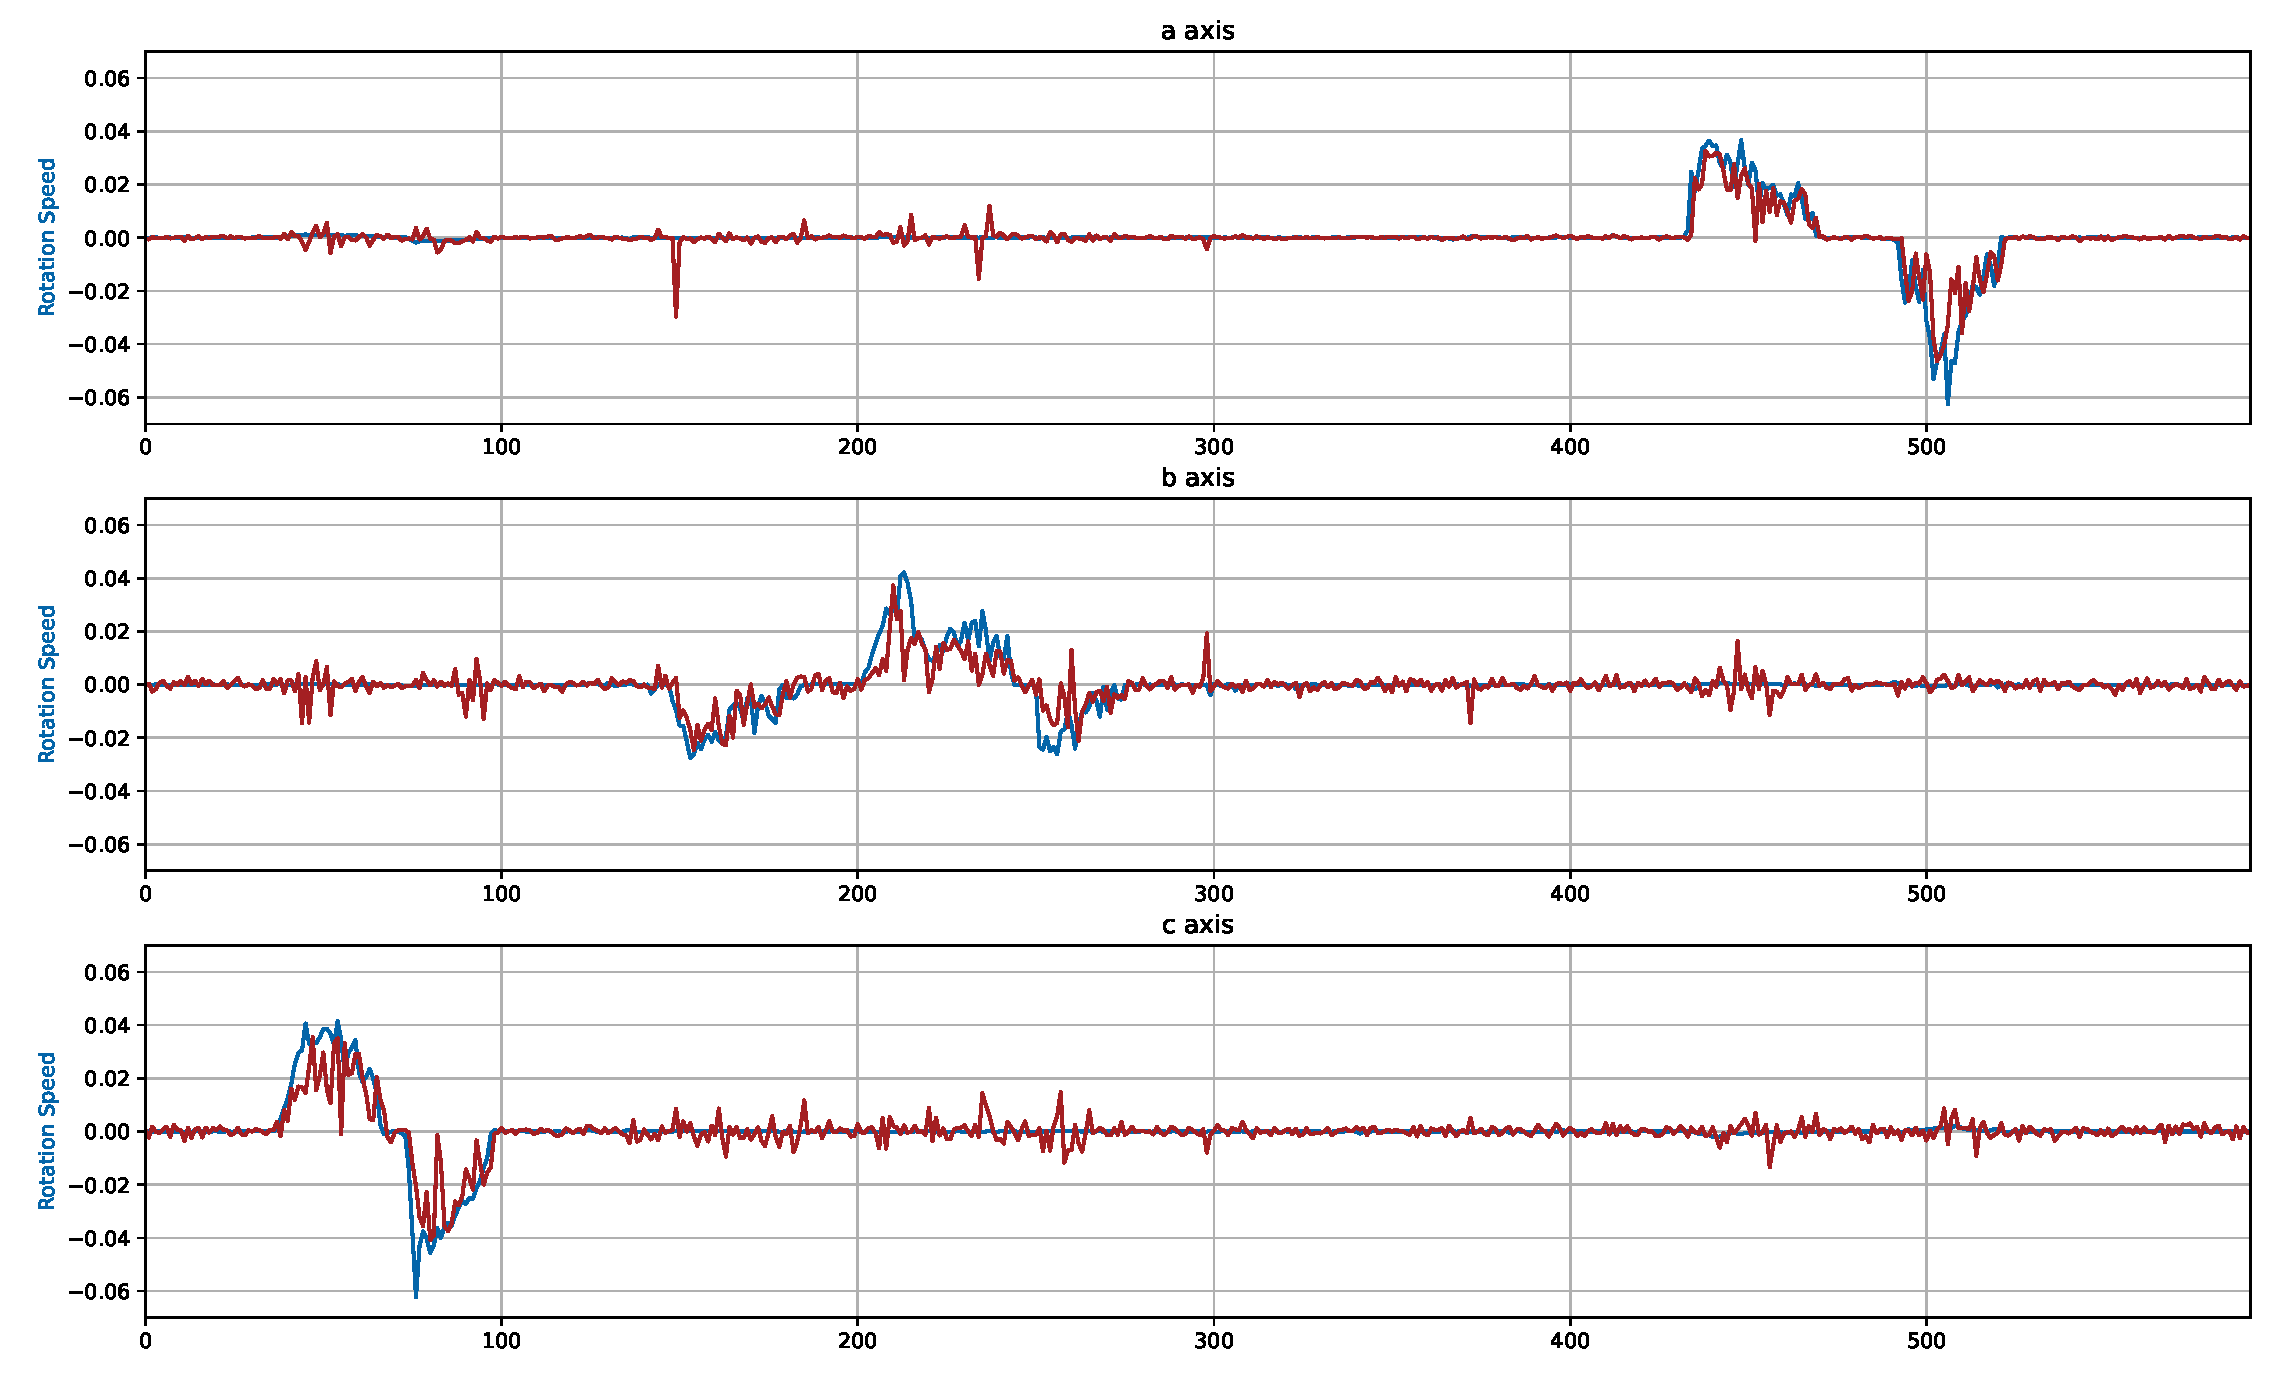
\includegraphics[width=1.0\textwidth]{images/tof_rotation_measurement.eps}
  \caption{The individual axis of the ToF rotation quaternion in red plotted against the gyroscope quaternion in blue. The camera head got rotated in each direction after another, first sideways around the $c$-axis, then downwards and upwards around the $b$-axis and at last tilted around the $a$-axis. The plotted values resemble imaginary parts of a quaternion and are therefore without units.}
  \label{im:tof_rotation_measurement}
\end{figure}
The measurement on the motion estimation from the ToF camera shows significant noise, especially on the rotation alongside the b- and c-axis, and does not entirely follow the gyroscope curve in blue. Nevertheless, measurement shows the proof of concept.
\subsection{Translation from ToF camera}
\label{sec:translation_tof_rotation}
Like for the rotation measurement, the translation is measured against the IMU. In the case of translation, the acceleration data from the IMU is compared to the translation estimation of the ToF camera. The camera is moved on a toy rail in $x$- and $y$-directions. Motion along the $z$-axis is not measured, as its priniciple is the same as for the $y$-direction. The translation cannot be measured in one take as the railway needs to be moved for the different axis.\\
Alongside the $x$-axis, the camera moves closer to the objects in the viewfinder, alongside the $y$-axis, the camera moves perpendicular. Note that these measurements are already in $xyz$-notation, as the orientation was corrected. As the camera did not rotate during these measurements, the values are equivalent to the $abc$-notation. The camera was slid from its origin to the front, respectively to the side, and to its origin twice on each run. The first motion was kept fast, the second motion was kept slow. The length of the track is about 0.5 m in both directions.\\
As visible in the Figures \ref{im:tof_translation_measurement_x} and \ref{im:tof_translation_measurement_y} on the next page, the velocity data from the ToF camera shows significant noise, but the motion is detected correctly.
\begin{figure}[H]
  \centering
  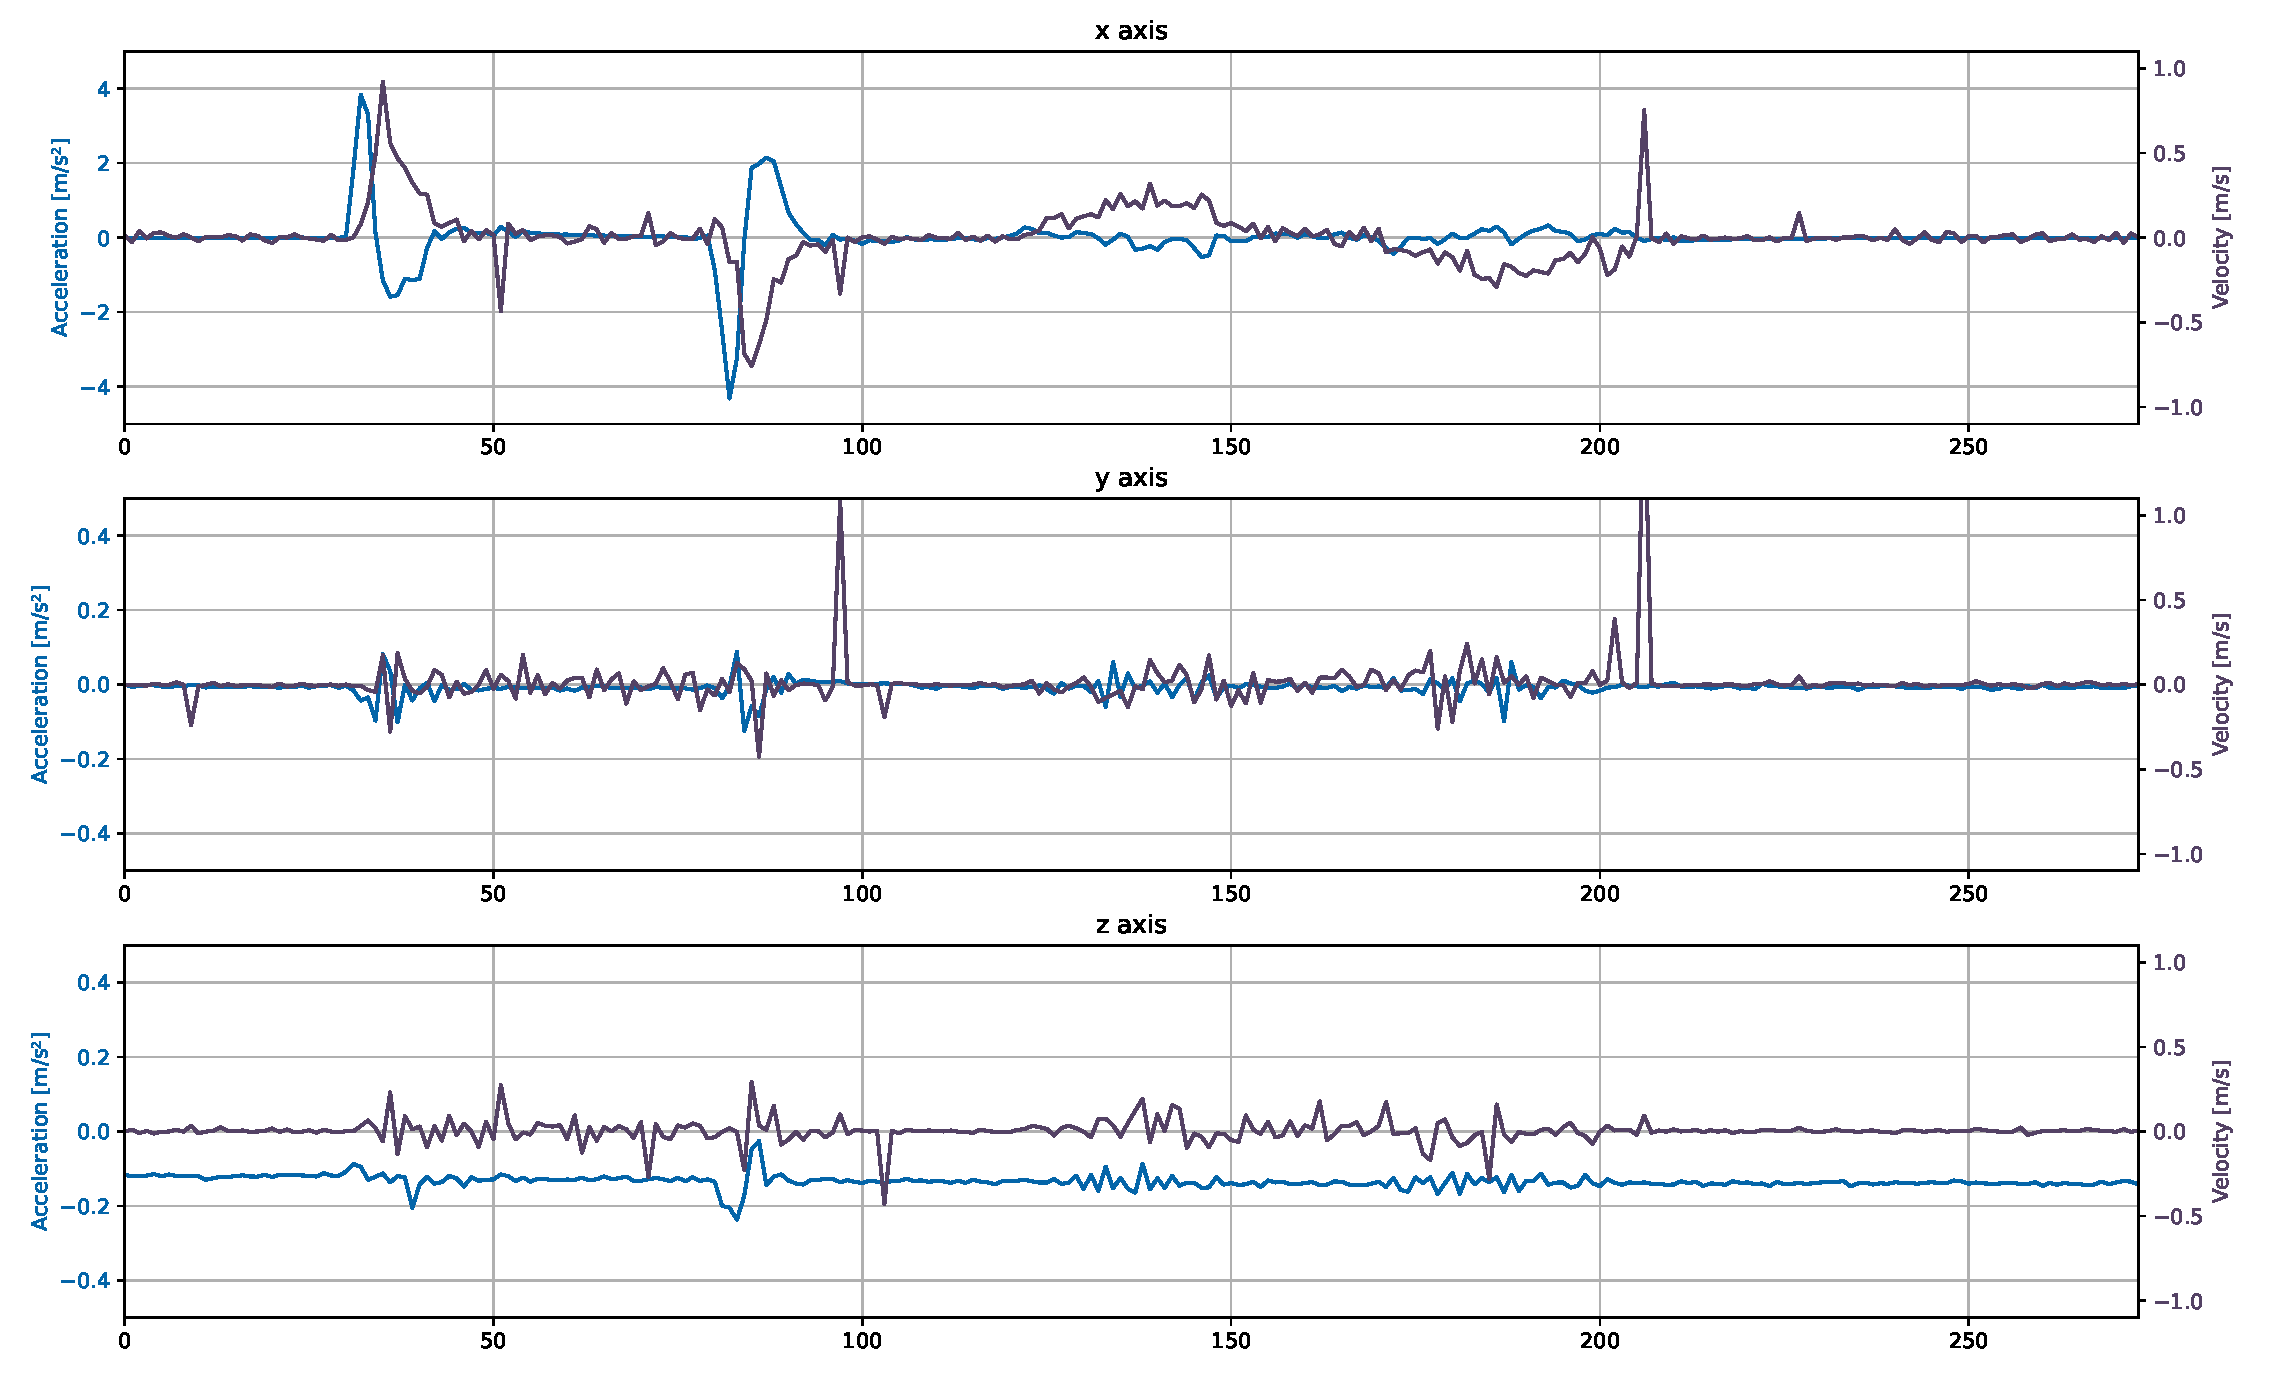
\includegraphics[width=1.0\textwidth]{images/tof_translation_measurement_x.eps}
  \caption{Raw measurement of the translation alongside the x-axis. Before and around frame 50, the camera is slid fast forward, kept in pause just to slide back before reaching frame number 100. After frame 100 and before frame 220, the same motion is repeated but slower. Blue is the acceleration from the IMU and purple the velocity from the TOF sensor.}
  \label{im:tof_translation_measurement_x}
\end{figure}
\begin{figure}[H]
  \centering
  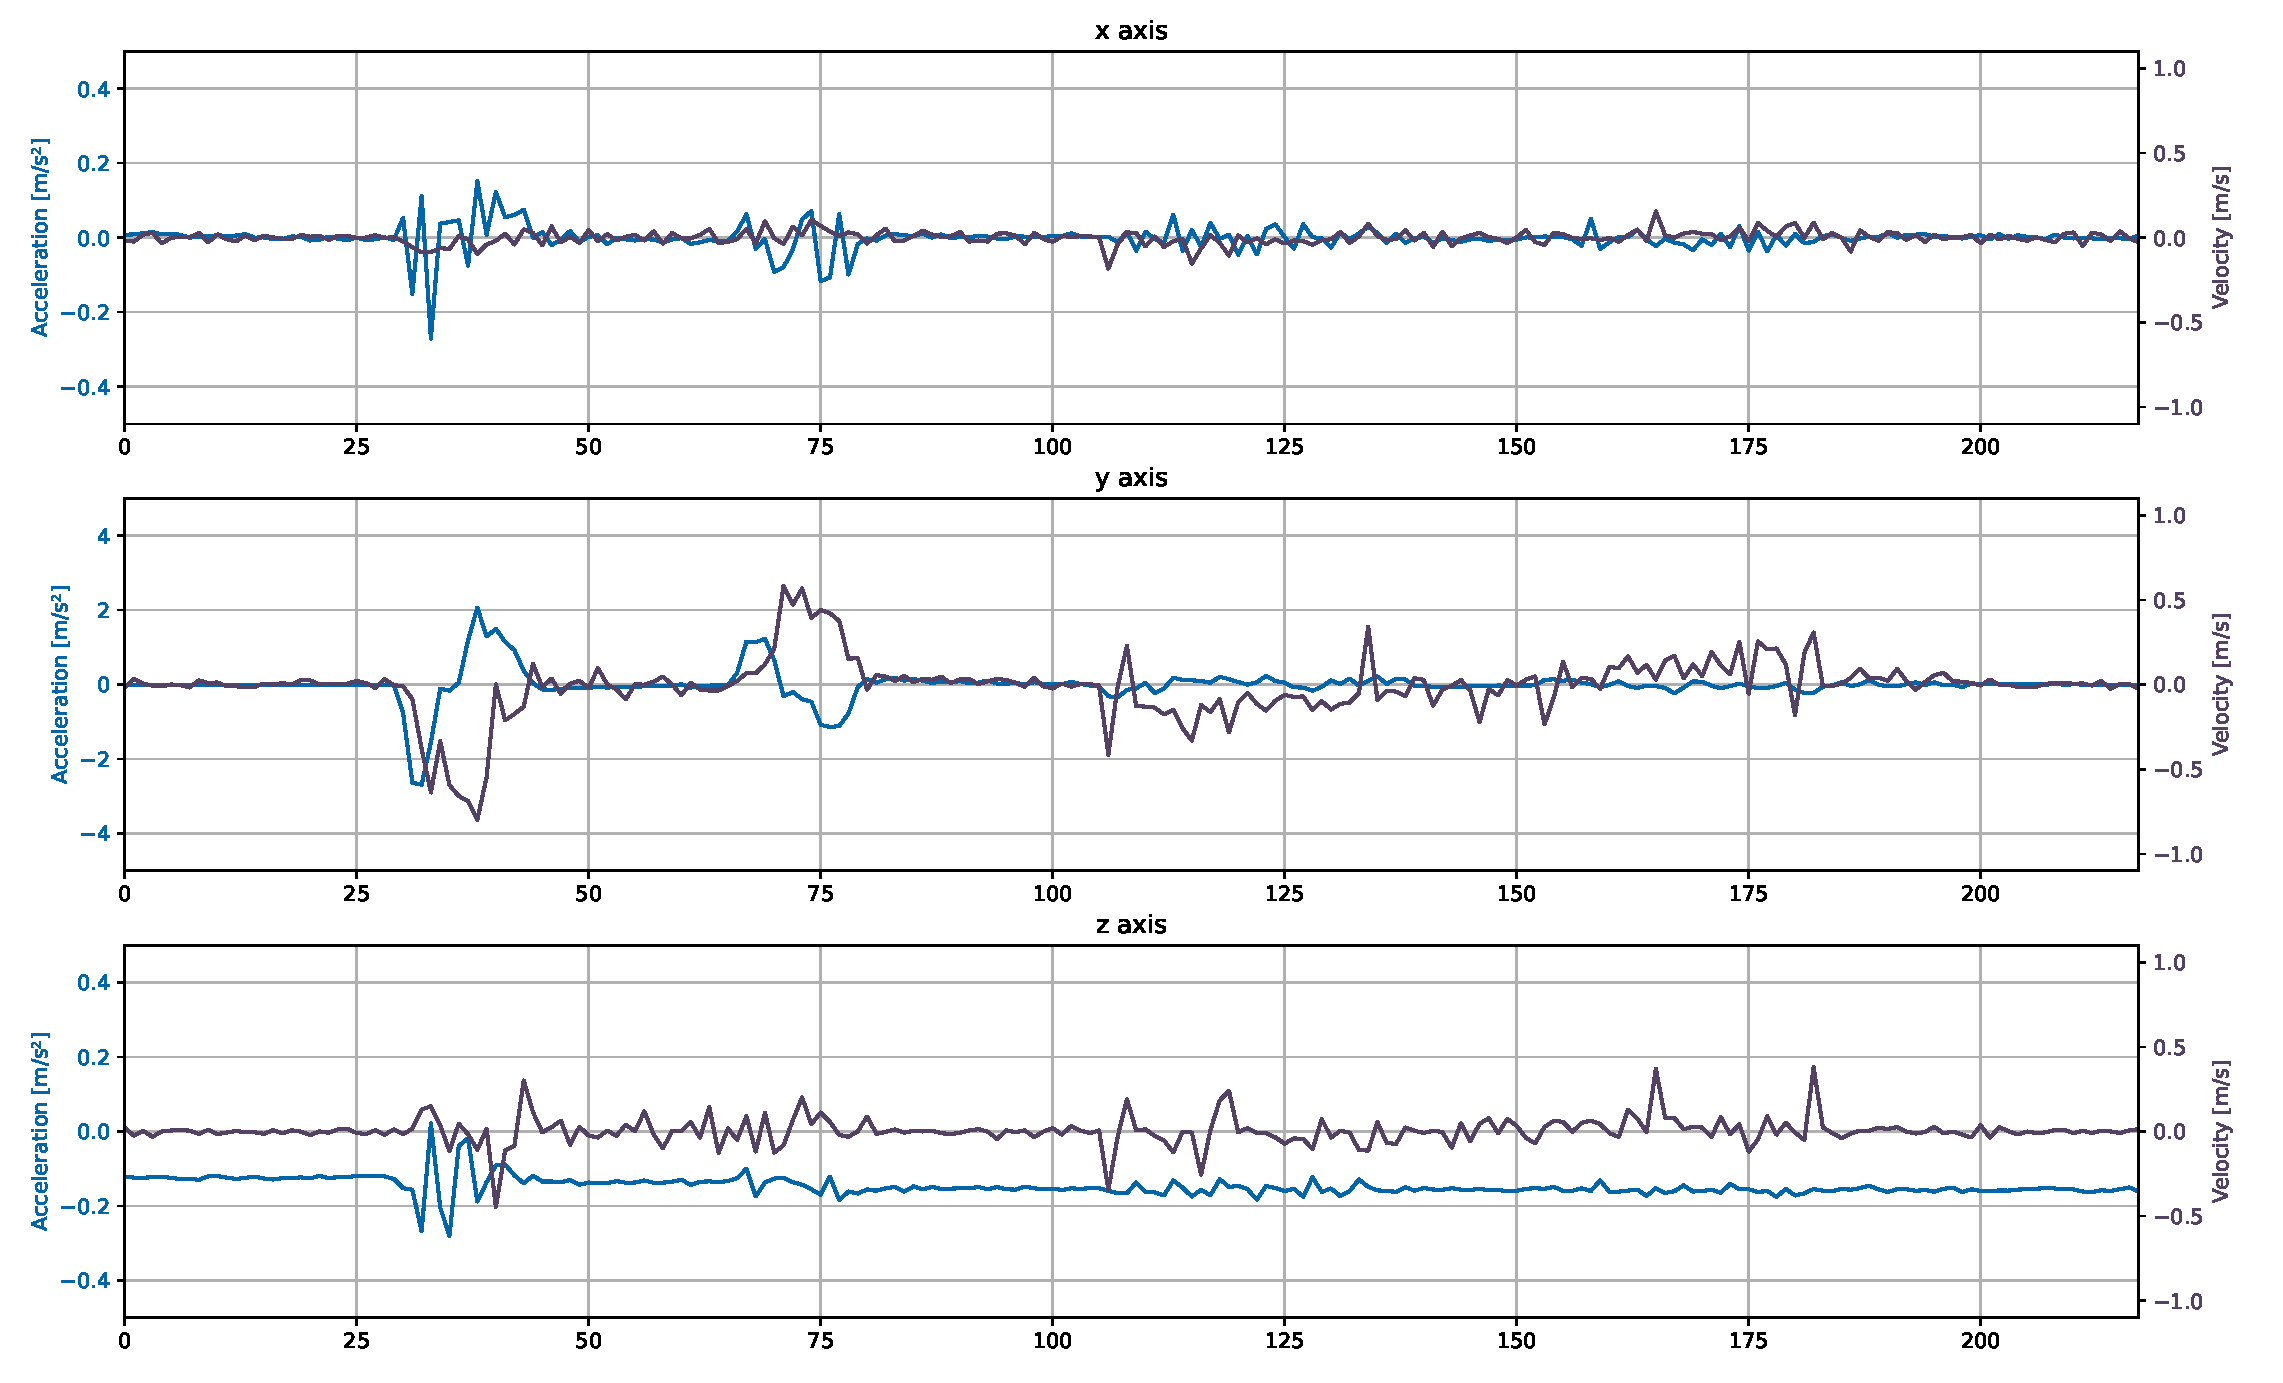
\includegraphics[width=1.0\textwidth]{images/tof_translation_measurement_y.eps}
  \caption{Raw measurement of the translation alongside the y-axis. Between the frames 25 and 50, the camera is slid to the right, kept there and slid back to the origin around frame 75. The motion is repeated slower after frame 100 and before 200. Blue is the acceleration and purple the velocity. Note how noise increased on the other axis, while the camera was in motion.}
  \label{im:tof_translation_measurement_y}
\end{figure}
Raw integration of the ToF velocity values gives insight into the measurement's quality. As visible in Figure \ref{im:tof_translation_measurement_integrated}, the data reconstructs the linear motion in both directions, even though it gets jagged by noise as expected. Noteable outliers, like at the end of the second motion on the x-axis, induce larger errors. 
\begin{figure}[H]
  \centering
  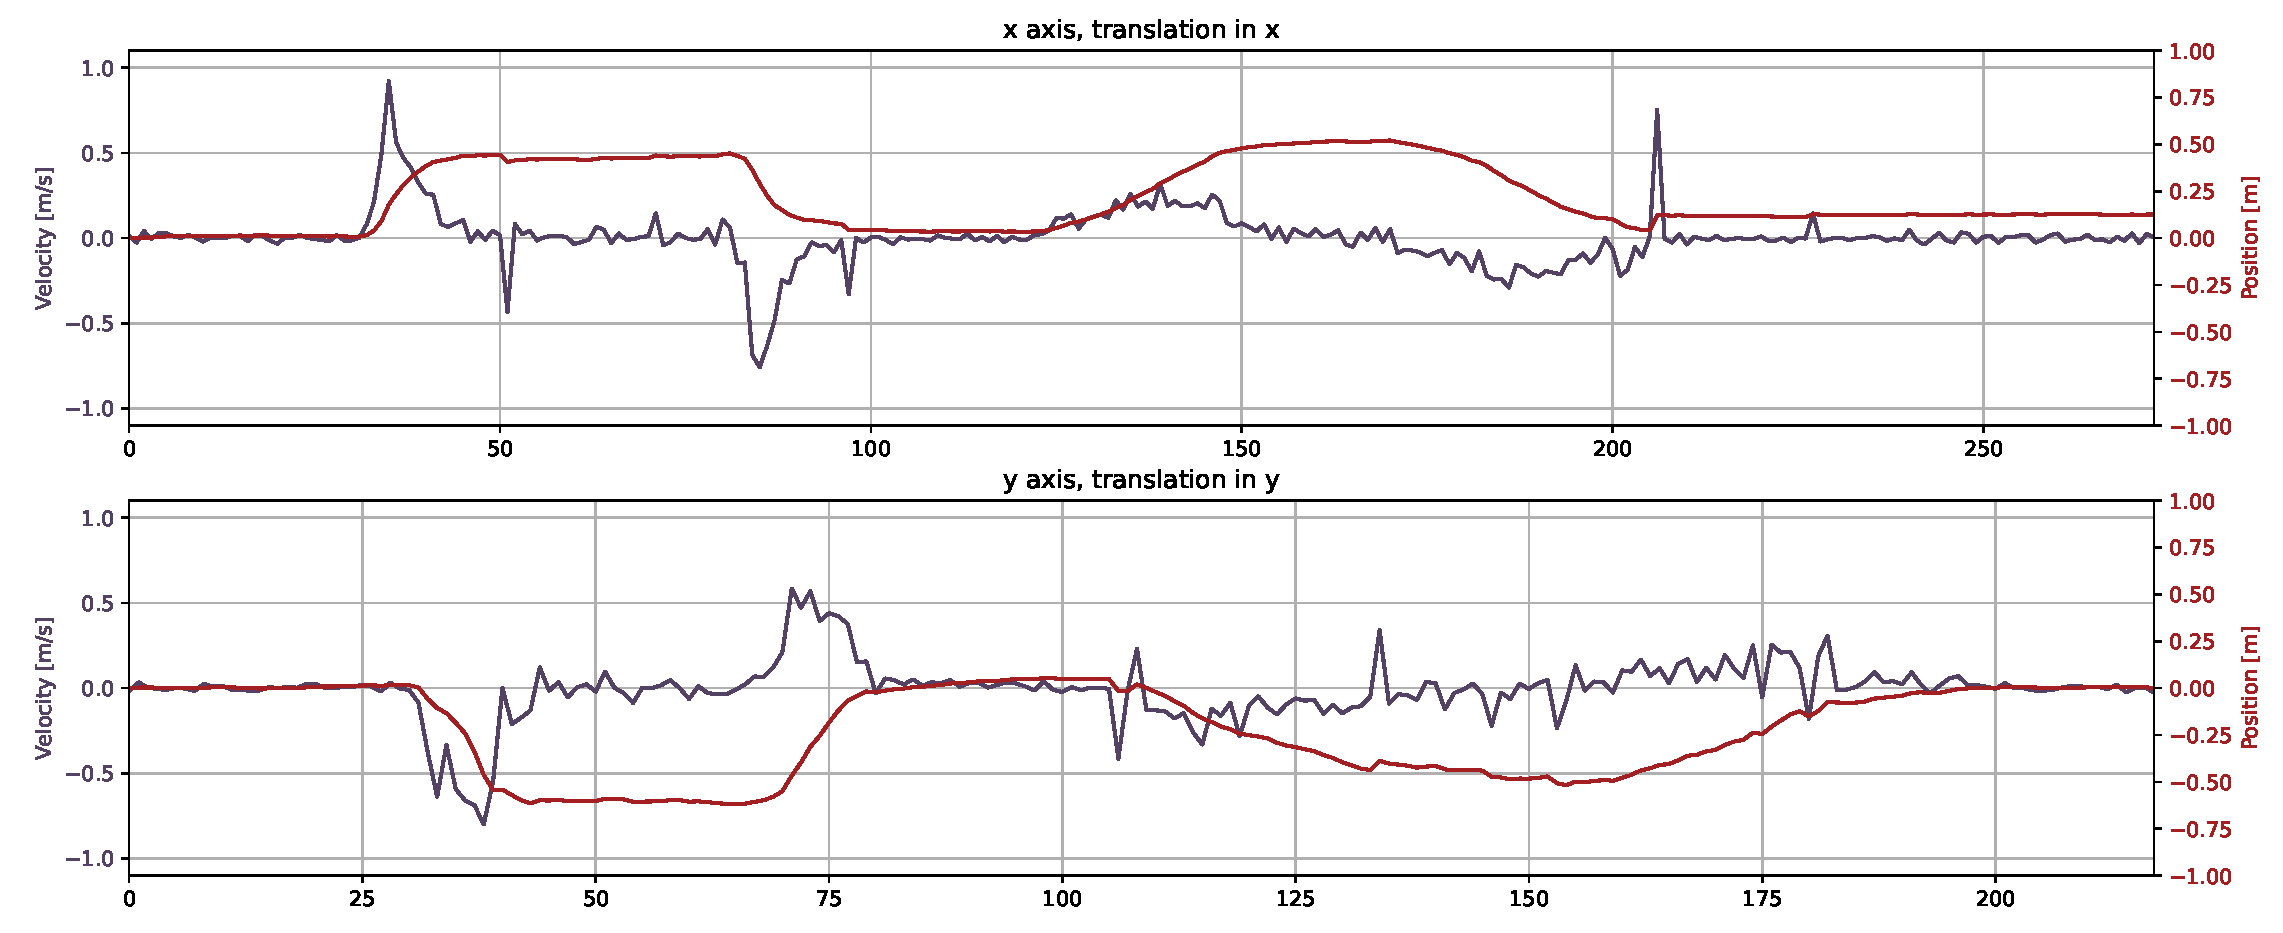
\includegraphics[width=1.0\textwidth]{images/tof_translation_measurement_integrated.eps}
  \caption{Raw integration of the relevant axis in both translations of the ToF velocity data. Purple is the velocity from the ToF camera and red its integration.}
  \label{im:tof_translation_measurement_integrated}
\end{figure} 
\section{Inertial Measurement Unit}
\label{sec:IMU_results}
The IMU contains a gyroscope and an accelerometer, whose data inputs the Kalman filter. While the comparison to the rotation estimation from the ToF camera already covered the gyroscope in Section \ref{sec:results_tof_rotation}, the accelerometer data requires more profound analysis.
\subsection{Accelerometer}
\label{sec:accel_results}
An accelerometer within the gravitational field of the earth will always measure the earth's gravitational pull in addition to other accelerations. The accelerometer needs calibration on each axis to compensate for the gravitational force, so the subtraction of $\vec{g}$ works in any orientation. Experimentation with the accelerometer showed that a hysteresis did prevent the accelerometer from reaching zero or $\vec{g}$ when standing still, depending on prior rotation. The hysteresis leads to a tiny offset on the acceleration, which causes an integrated velocity and devastatingly affects the further integrated position, as visible in Figure \ref{im:accelometer_integrated} on the next page. The aforementioned offset is visible \ref{im:tof_translation_measurement_x} and \ref{im:tof_translation_measurement_y} on the z-axis, thanks to the narrowed scale.\\
The added offset error worsens the drift compared to the simulation in Section \ref{sec:Kalmanfilter} dramatically. The integration to the velocity draws a smoother curve, than compared to the raw data of the ToF camera, but a drift is present. The third row of Figure \ref{im:accelometer_integrated} shows the critical drift, if the gravitational pull is not compensated entirely. The data for the third plot was recorded during the measurement of the motion alongside the x-axis.
\begin{figure}[H]
  \centering
  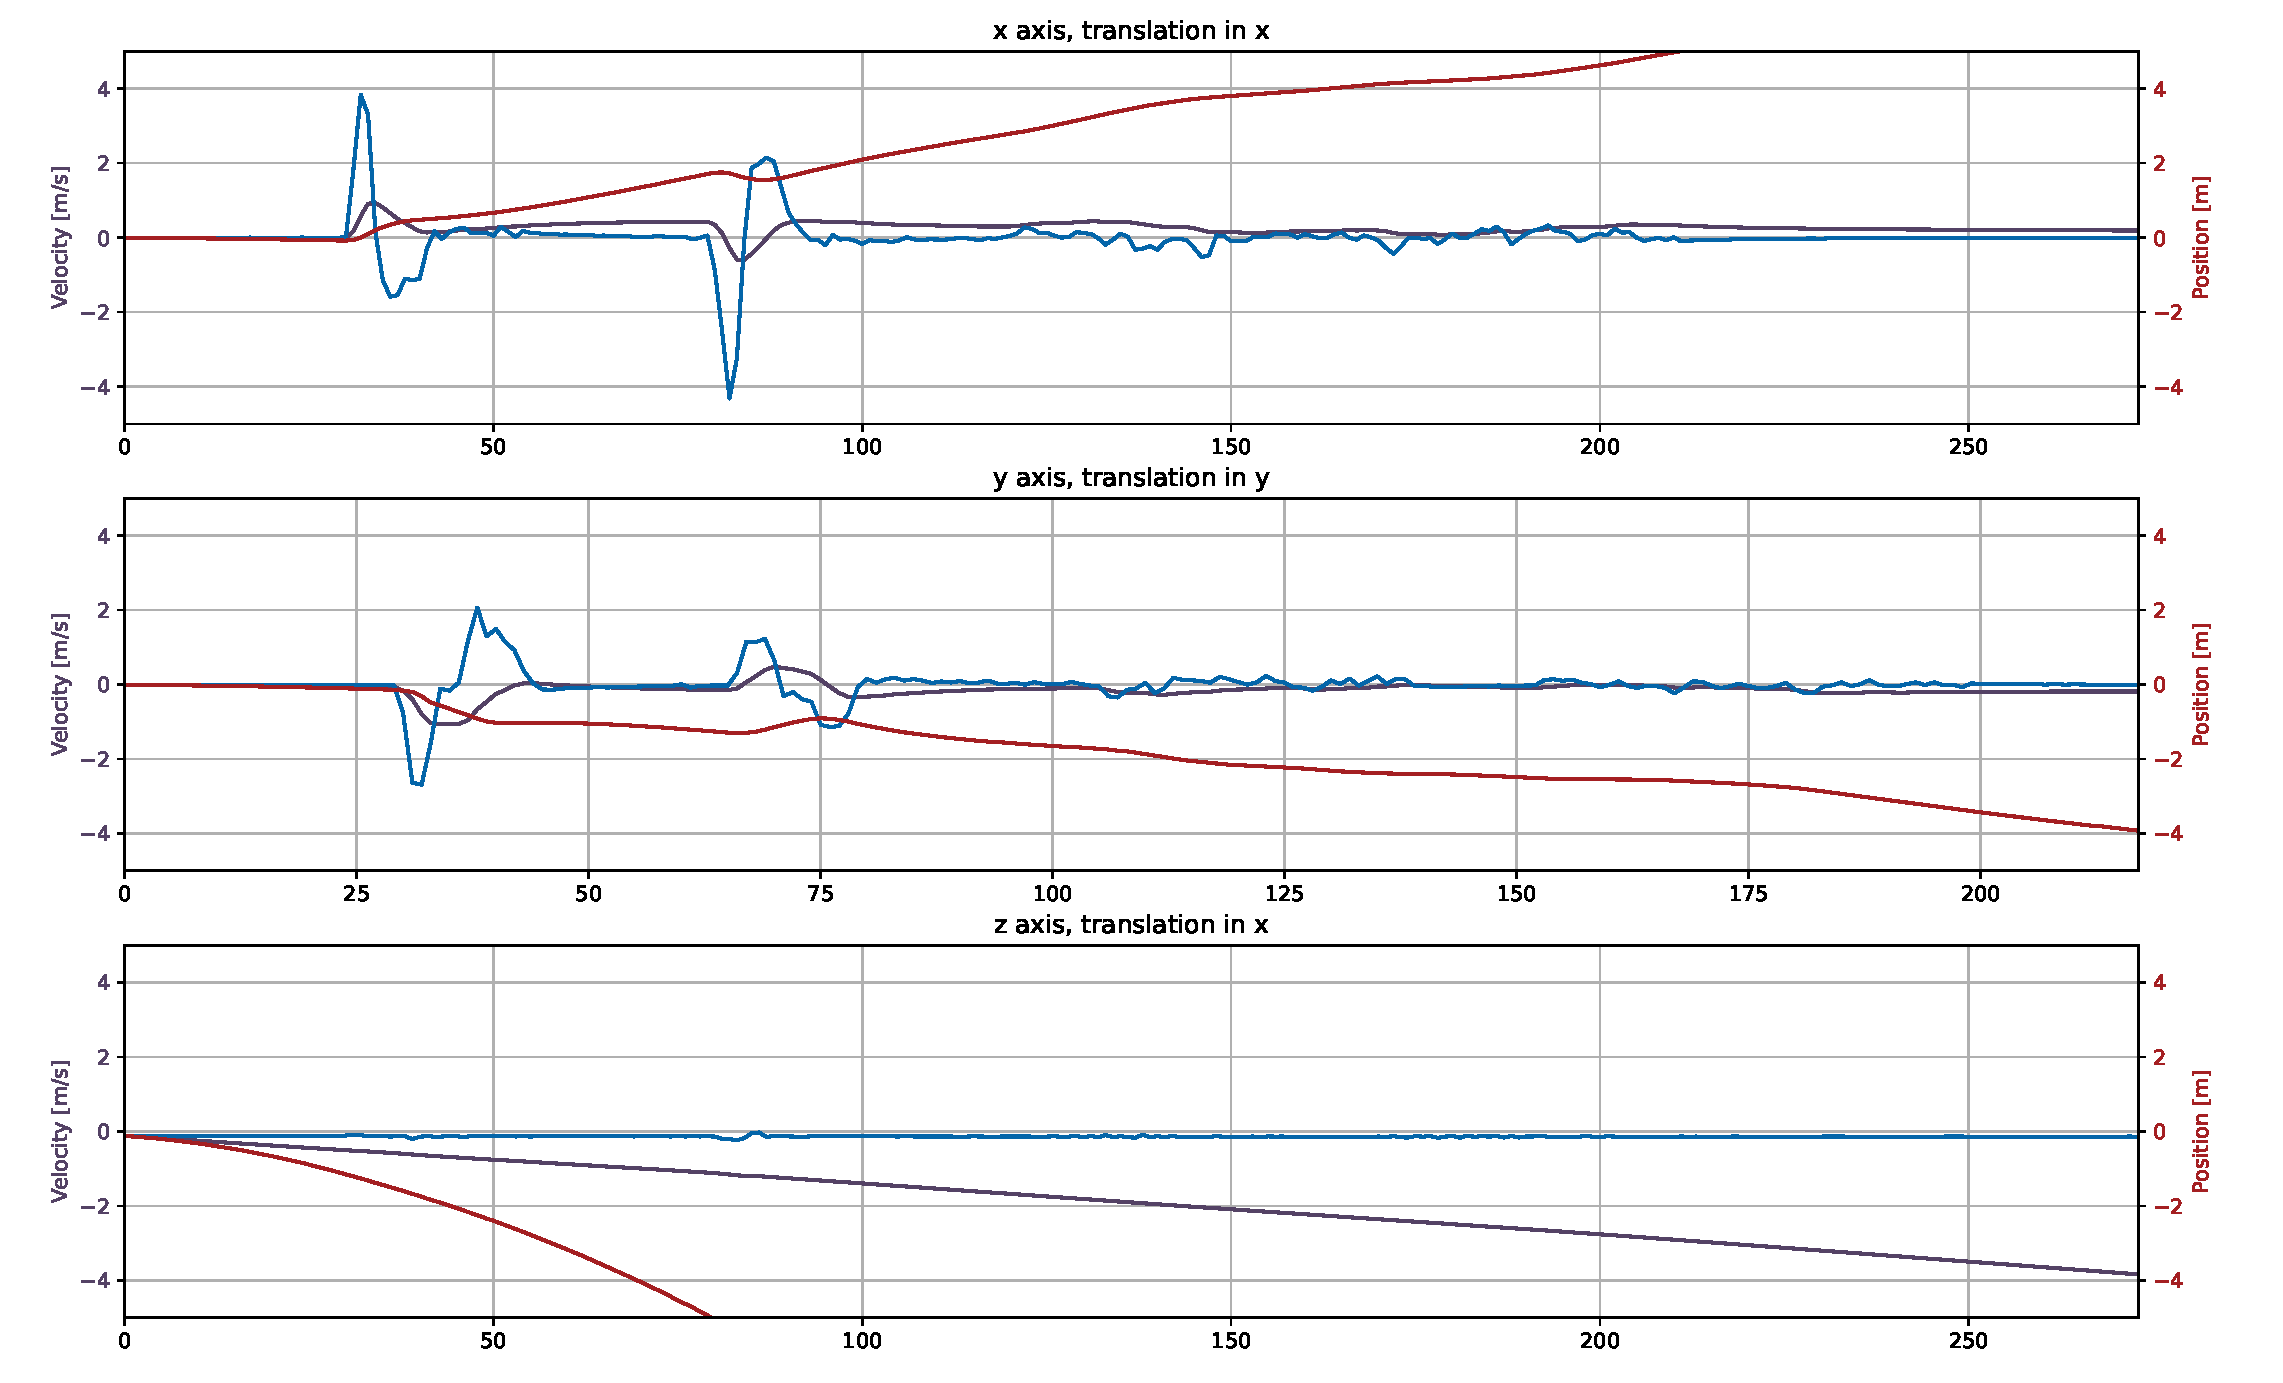
\includegraphics[width=1.0\textwidth]{images/accelerometer_translation_drift.eps}
  \caption{Integrations of the accelerometer data alongside relevant axis in both translations. Blue is the acceleration, purple the velocity (single integration) and red the position (double integration).}
  \label{im:accelometer_integrated}
\end{figure} 
\section{Kalman Filter}
\label{sec:kalman_results}
The Kalman filter combines the known motion model of the camera head with the measurement uncertainties and the raw input data from the ToF camera and the IMU. The only coupling between the rotation and the translation is the transformation from ABC-coordinates to the XYZ-space.
\subsection{Rotation}
\label{sec:kalman_rotation_results}
As mentioned in Section \ref{sec:results_tof_rotation}, the gyroscope and the ToF camera generate a rotation speed of comparable magnitude and shape. The gyroscope data is less distorted by noise, therefore the motion model can rely more heavily on this data source.\\
The Kalman filter smoothes data for the rotational speed through its model function and calculates the rotation from there. Additional to the gyroscope and the ToF camera, the drift compensation with the accelerometer stabilizes the values when the camera head is stationary.\\ 
In the comparison of the output of the Kalman filter against the sensory data, the strong weight towards the gyroscope becomes apparent, as shown in Figure \ref{im:meas_kalman_rotation}.\\
The shown result in Figure \ref{fig:rotation_demo} of the whole pipeline using only rotation data helps estimate the result's quality. The three rotation axes of the camera tripod do not intersect with the recording Raspberry Pi camera, thus, the 3D object moving in the image was expected. While the gyroscope's rotation axes intersect in the housing of the IMU, the axes of the ToF camera intersect at the optical center of the lens. For better accuracy, these sensor- and camera displacements on the camera head require additional compensation. 
\begin{figure}[H]
  \centering
  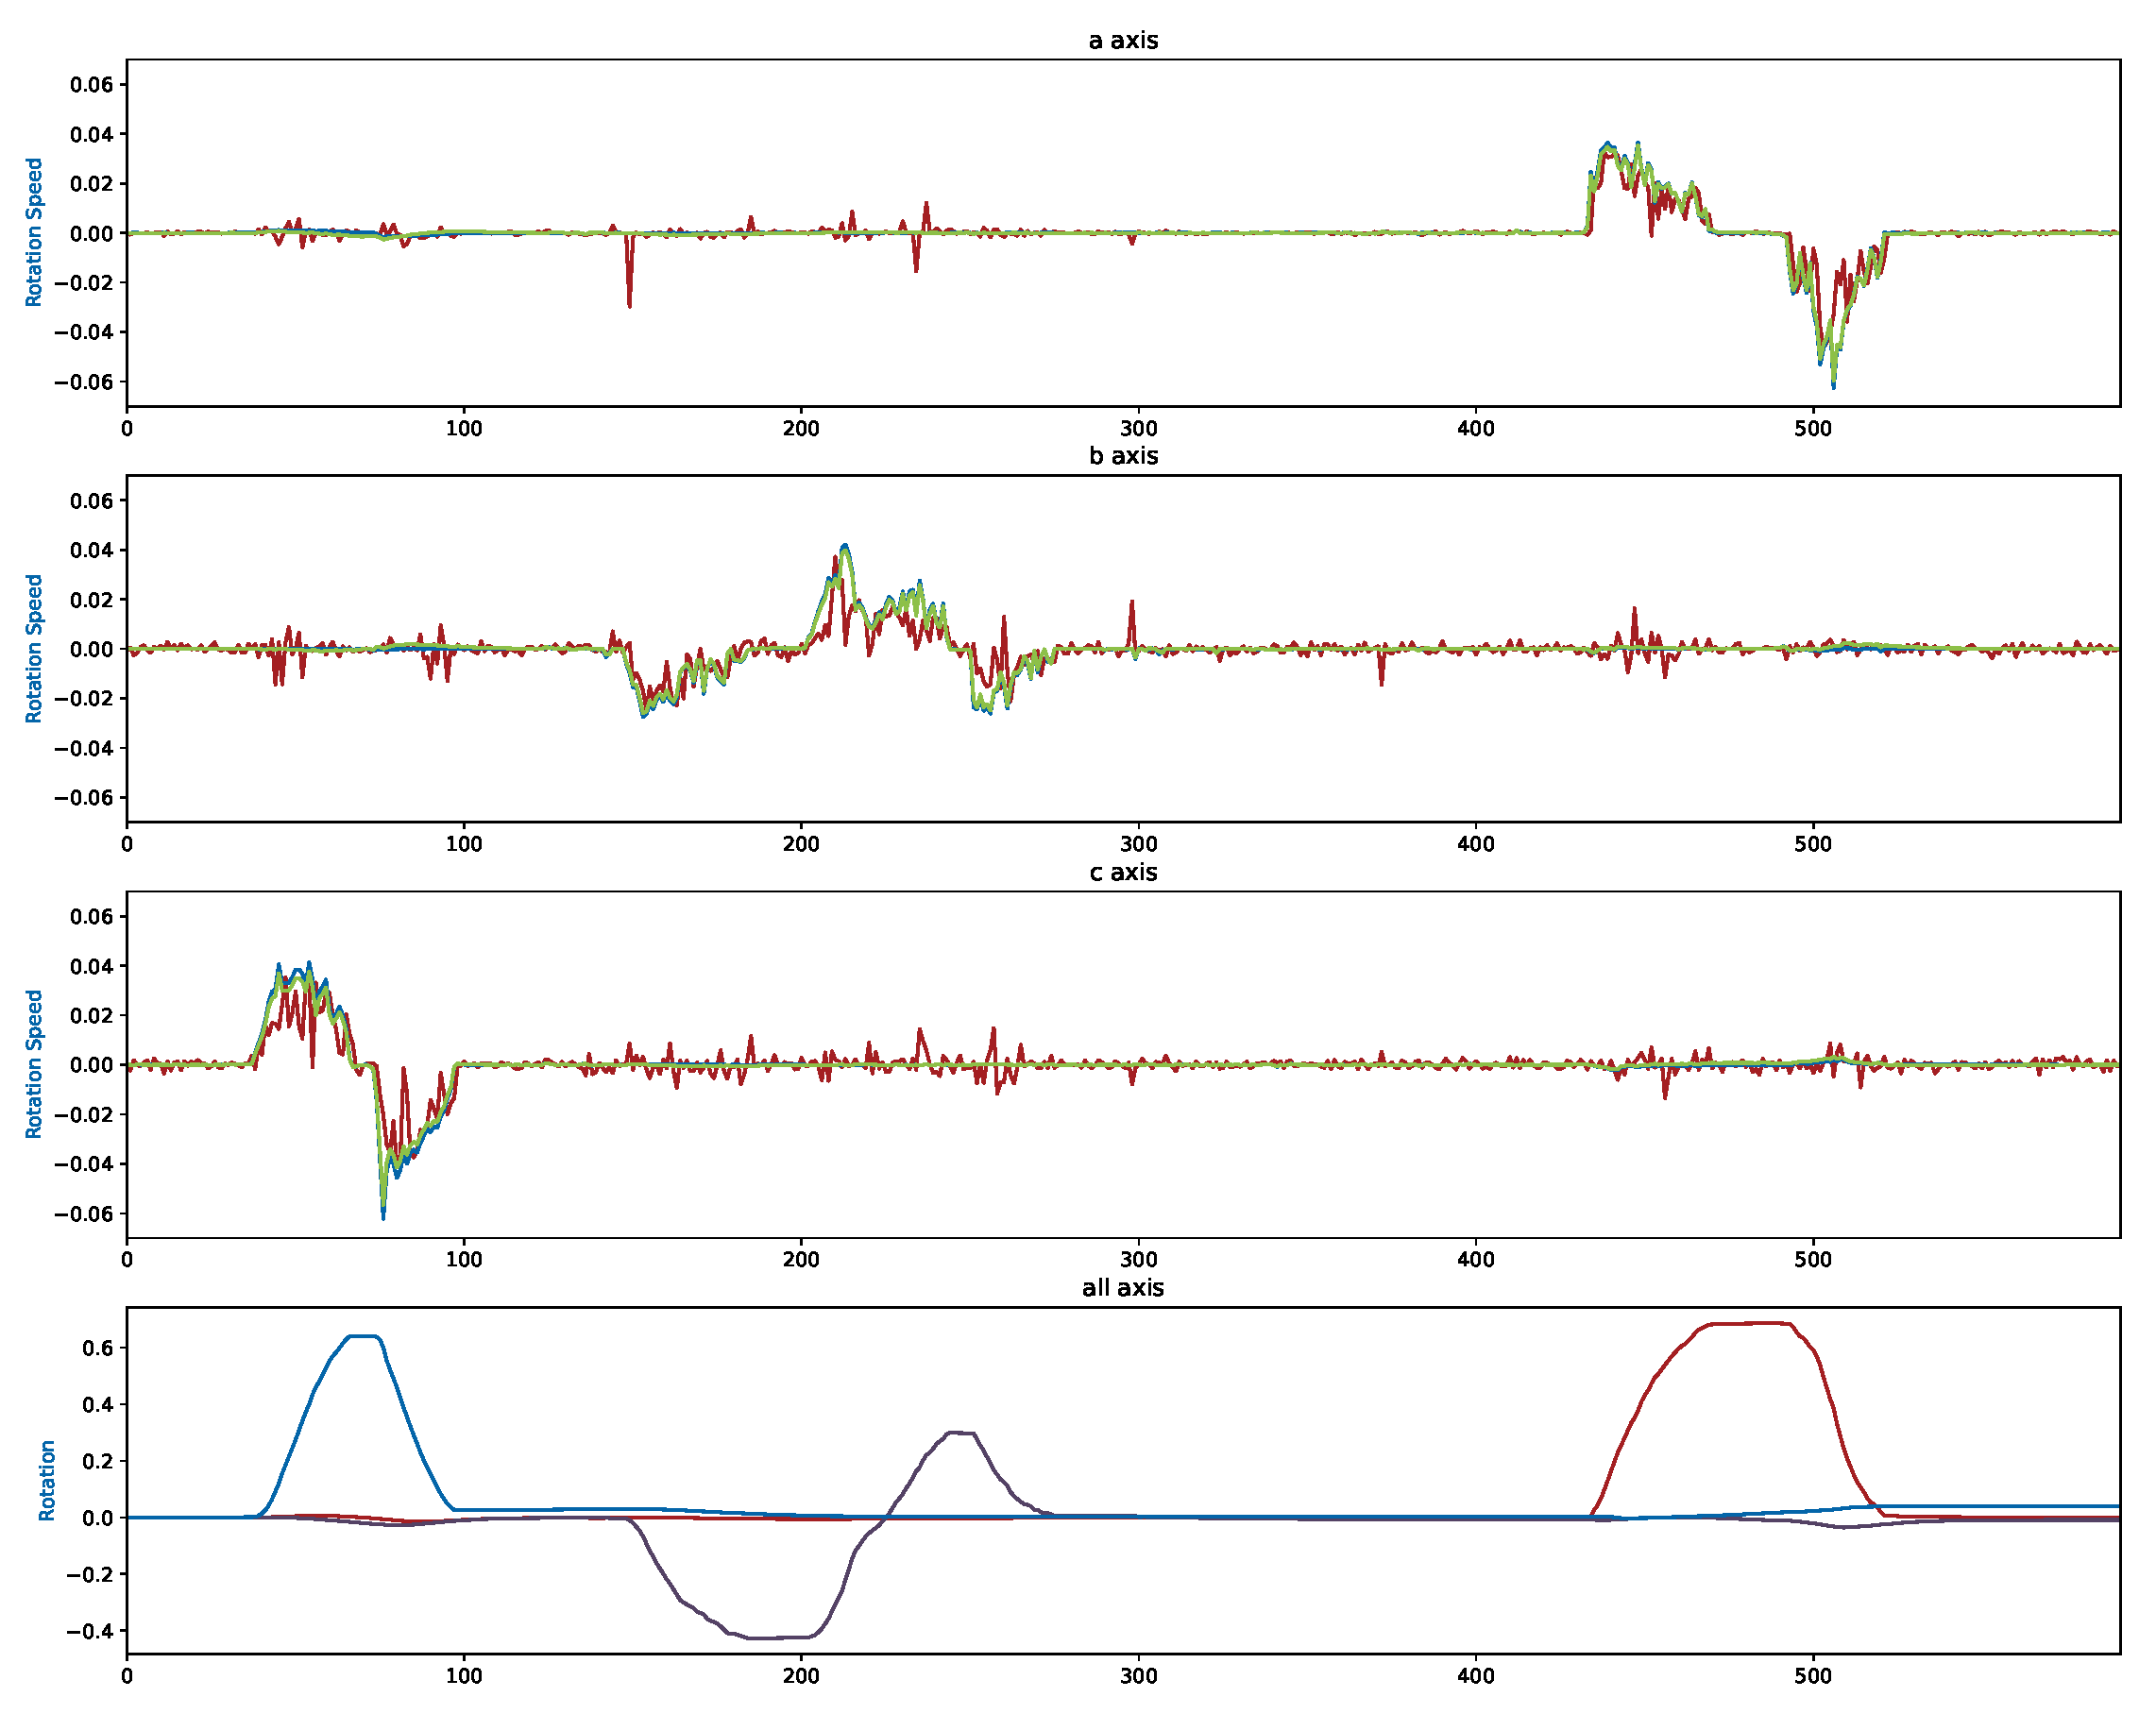
\includegraphics[width=1.0\textwidth]{images/meas_kalman_rotation.eps}
  \caption{The output of the Kalman filter is plotted in green, against the gyroscope data in blue and the ToF camera data in red in first three rows. The fourth row shows the calculated rotation. The a-axis in red, the b-axis in purple and the c-axis in blue.}
  \label{im:meas_kalman_rotation}
\end{figure} 
\begin{figure}[H]
  \centering
  \begin{minipage}[b]{0.47\textwidth}
    \includegraphics[scale=0.1115]{images/demo_rotation_init.png}
    \subcaption{Initial situation}
    \label{fig:rotation_demo_init} 
  \end{minipage} % Hier darf keine Leerzeile zwischen den beiden Minipages liegen!
  \begin{minipage}[b]{0.47\textwidth}
    \includegraphics[scale=0.1115]{images/demo_rotation_rotated.png} 
    \subcaption{After rotation}
    \label{fig:rotation_demo_rotated} 
  \end{minipage}
  \caption{Demonstration of the rotation against the camera image with the moving projection. The displacement of the rectangle inside the picture frame is a result of the Raspberry Pi camera facing translational motion when rotated on the camera tripod.}
  \label{fig:rotation_demo}
\end{figure}
\subsection{Translation}
\label{sec:kalman_translation_results}
 Figure \ref{im:meas_kalman_translation} shows the output of the Kalman filter in green against the data from the accelerometer and the ToF camera. Without other input to compare against, the Kalman filter follows the accelerometer directly. The accelerometer's integration curve compares directly against the raw ToF camera data and the Kalman filter output on the velocity. Further integration allows the comparison with the positional data.\\
The accelerometer impacts the filter output, rendering it worse than the raw integration of the ToF camera. The Kalman velocity output is significantly worse than in the simulation, the proposed integration on this output, to get even better positional data fails.
\begin{figure}[H]
  \centering
  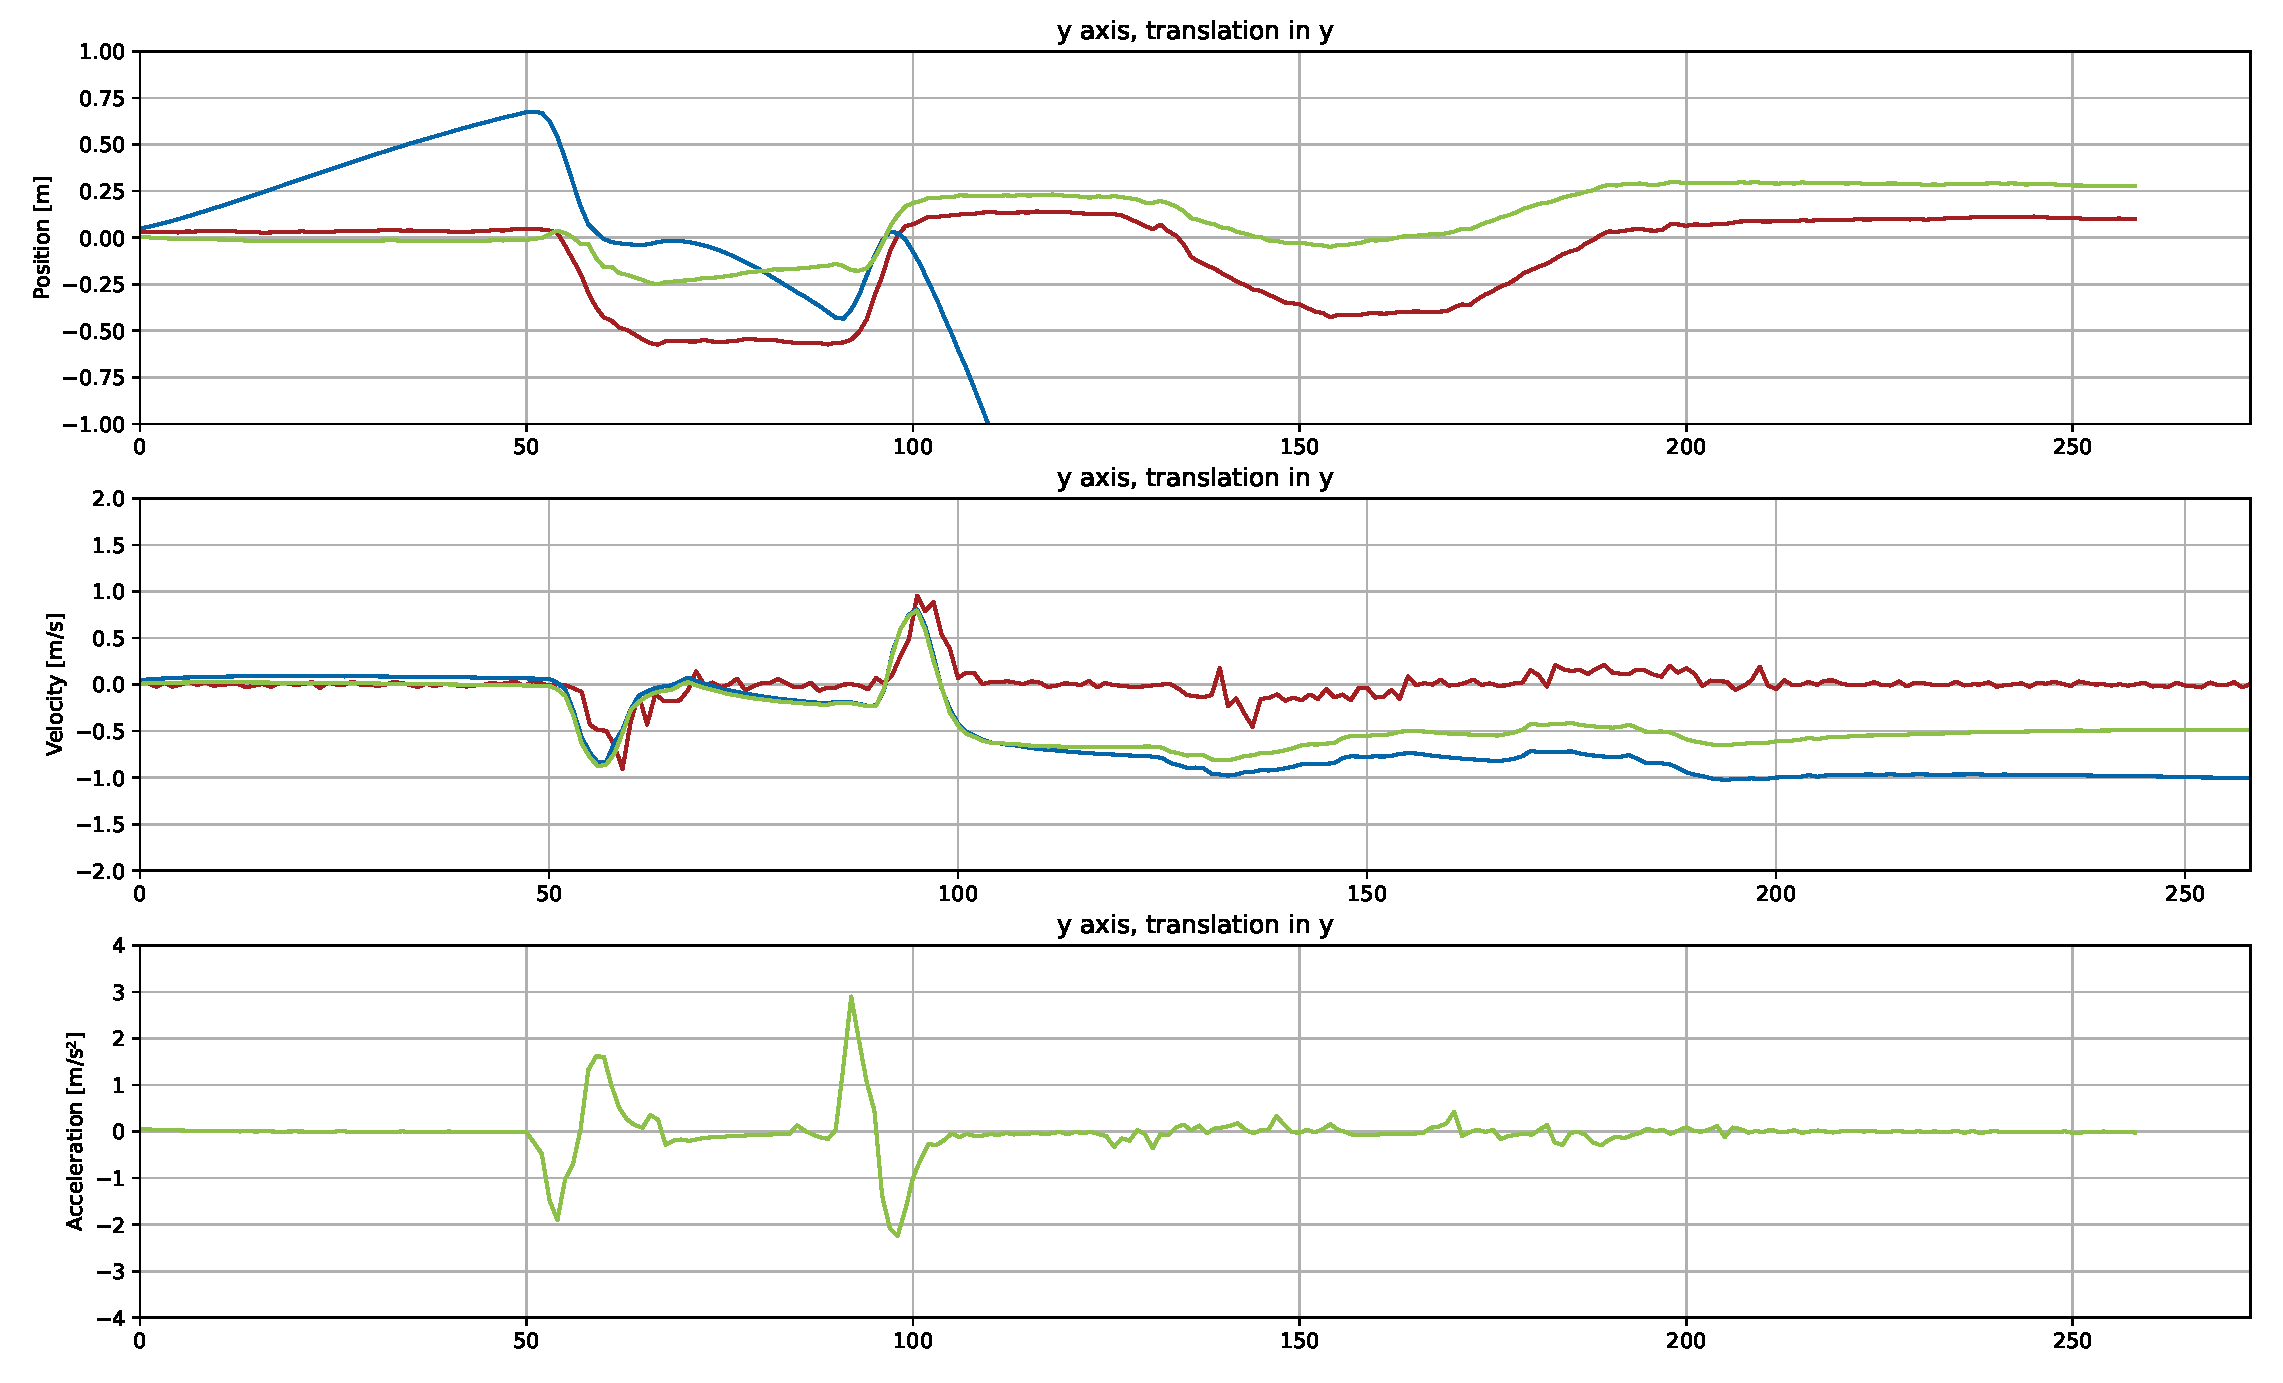
\includegraphics[width=1.0\textwidth]{images/measurement_kalman_translation.eps}
  \caption{Motion in y direction. Blue lines are data from the accelerometer and its integrations, red are the velocity from the ToF camera and its integration and in green are the different Kalman outputs. }
  \label{im:meas_kalman_translation}
\end{figure} 
